\documentclass[preprint,5p,times,authoryear]{elsarticle}

\usepackage{wrapfig}
\usepackage[font=small]{caption}
\usepackage[hyperref,usenames,svgnames,dvipsnam]{xcolor}
\usepackage[labelformat=empty]{subcaption}
\usepackage{amsmath}
\usepackage{mathtools}
\usepackage{bm}
\usepackage{breqn}
\usepackage{geometry}
%\usepackage{url}
\usepackage{booktabs}
\usepackage{multirow}
%\usepackage{stfloats}
\usepackage{xfrac}
\usepackage{units}
\usepackage{tabularx}
\usepackage{dblfloatfix}

\usepackage{array}
\newcolumntype{P}[1]{>{\centering\arraybackslash}p{#1}}
\newcolumntype{M}[1]{>{\centering\arraybackslash}m{#1}}

\usepackage{siunitx}
\sisetup{separate-uncertainty}%,range-units = single}
\DeclareSIUnit\year{yr}

\usepackage[colorlinks]{hyperref}

\bibliographystyle{model2-names}\biboptions{authoryear}

\journal{Icarus}

\begin{document}

\hypersetup{
     allcolors = MidnightBlue
}

\urlstyle{same}

\begin{frontmatter}

\title{Numerically Modelling Ocean Dissipation in Titan and Enceladus: A Comparison of Rayleigh and Bottom Drag}

\author[label1]{Hamish C. F. C. Hay\corref{cor1}}
\ead{hhay@lpl.arizona.edu}
\author[label1]{Isamu Matsuyama}
\address[label1]{Lunar and Planetary Laboratory, University of Arizona, Tucson, AZ 85719, United States}

\cortext[cor1]{Corresponding author}

\begin{keyword}
Satellites \sep Ocean Tides \sep Bottom drag\sep Titan \sep Enceladus 
\end{keyword}

\begin{abstract}

Icy satellites that contain subsurface oceans require sufficient thermal energy to prevent the liquid portion of their interiors from freezing. We develop a numerical finite difference model to solve the Laplace Tidal Equations on a sphere in order to simulate tidal flow and thermal energy dissipation in these oceans, neglecting the presence of an icy lid. The model is applied to Titan and Enceladus, where we explore how Rayleigh (linear) and bottom (quadratic) drag terms affect dissipation. The latter drag regime can only be applied numerically. We find excellent agreement between our results and recent analytical work. Obliquity tide Rossby-wave resonant features become independent of ocean thickness under the bottom drag regime for thick oceans. We show that for Titan, dissipation from this Rossby-wave resonance can act to dampen the rate of outward orbital migration by up to \SI{40}{\percent} for Earth-like values of bottom drag coefficient. Gravity-wave resonances can act to cause inward migration, although this is unlikely due to the thin oceans required to form such resonances. The same is true of all Eccentricity tide resonances on Enceladus, such that dissipation in our model is negligible for thick oceans under the bottom drag regime.  

\end{abstract}
\end{frontmatter}

\newpage
\section{Introduction}

\hbadness=10000
\vbadness=10000

The primary source of heat generation in the outer Solar System icy satellites is energy lost via tidal dissipation. A result of this heating is the formation and potentially long term stable existence of global subsurface oceans, as has already been confirmed in several of the icy satellites. Europa has been shown to have an induced magnetic field consistent with a global layer of salty, liquid water beneath its surface \citep{zimmer2000subsurface, kivelson2000galileo, hand2007empirical}. This is also the case with Ganymede and Callisto, although these liquid oceans are likely to exist at least a few hundred kilometers beneath the surface \citep{zimmer2000subsurface, kivelson2000galileo}. Saturn's largest moon, Titan, has been interpreted to have a conductive liquid layer beneath its surface due a Schumann-like resonance \citep{beghin2010titan}, and this is supported by measurements of its mean moment of inertia \citep{bills2011rotational}. Enceladus also shows signs of a liquid ocean confined to its southern hemisphere. Evidence for this includes emission and composition of cryovolcanic plumes from a series of tidally induced shear faults over its south pole \citep{hansen2011composition}, as well as a detected negative mass anomaly consistent with a subsurface ocean \citep{iess2014gravity}. 

Despite this overwhelming evidence and abundance of subsurface oceans in the icy satellites, previous tidal dissipation studies have not been able to account for the energy needed to sustain these oceans over time. Many of these studies have primarily focused on tidal dissipation in the solid regions of the satellite \citep[e.g.,][]{moore2000tidal, roberts2008tidal, beuthe2013spatial}, ignoring the effects of a subsurface ocean. This is somewhat surprising as ocean dissipation is expected to dominate energy loss in the system, as is the case for Earth.

Other previous works on tidal dissipation within the icy satellites have considered a rather idealised case with only a global surface ocean, completely ignoring the effects of a solid lid \citep{sagan1982tide, sears1995tidal, sohl1995tidal, tyler2008strong, matsuyama2014tidal}. By assuming that there is no solid lid, much of this work is not directly applicable to the icy satellites of the outer Solar System as they only have subsurface oceans. The presence of a solid lid is likely to dampen tidal dissipation in the liquid ocean, and thus it is important to examine the potential consequences that solid lids may have on tidal heating.

Tidal dissipation not only plays a role in the thermal evolution of the icy satellites, but but it also affects their rotational and orbital state. By studying and considering the effects of dissipation in the solid and liquid regions of the outer Solar System icy satellites, we hope to not only understand and help constrain their current thermal state and interior structure, but also how the satellite's interior, rotation and orbit has evolved over time. 

\section{Methodology}

This section describes some of the theory and methods involved in this work. The governing equations of the numerical model presented here are discussed in section \ref{subsec:LTE}. Following this, a description of the equations discretisation and the numerical scheme required to solve them are outlined in section \ref{subsec:model}.

\subsection{Laplace Tidal Equations \label{subsec:LTE}}

The equations of motion and mass conservation that describe ocean flow in the shallow water limit are called the Laplace Tidal Equations (LTE) (also known as the shallow water equations) \citep{lamb1932hydrodynamics}. The main assumption in their derivation is that radial (vertical) ocean flow is negligible when compared to lateral flow. This is indeed a good approximation for global oceans, where lateral flow spans a much greater distance than the depth of the ocean. The conservation of mass (eq. \ref{eq:mass}) and momentum (eq. \ref{eq:mom}) that make up the LTE, including both Rayleigh and bottom friction, are given as \citep{sears1995tidal,tyler2008strong,matsuyama2014tidal}:

%Adds vertical space between equations
%\setlength{\jot}{8pt}
%environment centres all equations

\vspace{-0.5cm}
\begin{gather}
\partial_t \eta + \nabla \cdot \left(h \bm{u}\right) = 0\, , \label{eq:mass}\\
\begin{aligned} 
\partial_t \bm{u} + 2 \bm{\Omega} \times \bm{u} + \alpha\bm{u} + \frac{c_D}{h} \left|\bm{u}\right| \bm{u}  + g \nabla \eta \\ = (1 + k_2 - h_2) \nabla U_2 \, . \label{eq:mom}\\
\end{aligned} 
\end{gather}

Equation \ref{eq:mass} consists of two terms. The first is the time rate of change of vertical sea surface displacement about some equilibrium level. $\eta$ denotes this displacement. The second term represents the divergence of the surface velocity vector, $\bm{u} \equiv (u, v)$, where $u$ and $v$ are the eastward and northward velocity components respectively. In our calculations, we assume the ocean's undisturbed depth, $h$, to be constant. 

The term on the right hand side of Equation \ref{eq:mom} is an applied force per unit mass. $\nabla U_2$ is the gradient of the degree-2 tidal potential (discussed in section ...). It is multiplied by Love's reduction factor involving the degree-2 tidal Love numbers, $k_2$ and $h_2$. Love's first number, $k_2$, is a proportionality constant accounting for the additional tidal potential due to the elastic redistribution of mass on the satellite. $h_2$, the second Love number, accounts for the tidal potential arising from solid body surface displacement of the satellite \citep{love1911some}.

The time derivative of velocity is given by the first term on the left hand side of the momentum equation. It is balanced by four other acceleration per unit mass terms on the left hand side. The first of these terms is the coriolis acceleration per unit mass, where $\Omega$ is the satellite's rotational angular velocity. Rayleigh and bottom friction are described in the next two terms, where $\alpha$ and $c_D$ are the Rayliegh (linear)and bottom (quadratic) friction coefficients respectively \citep{sears1995tidal,chen2013tidal}. The last term on the right hand side of Equation \ref{eq:mom} is the gravitational restoring acceleration per unit mass. It acts to balance changes in sea surface displacement, given by the gradient of equilibrium displacement, $\nabla \eta$ .

\subsection{Numerical Model \label{subsec:model}}

The numerical model outlined below is based on the models extensively discussed in \citet{zahel1973diurnalk,zahel1978influence} and \citet{sears1994tidal,sears1995tidal}. In this section we first provide a description of the numerical grid setup, before giving an overview of the finite difference scheme itself.

\subsubsection{Discretized Grid}

We made grid. 

\subsubsection{Finite Difference Expansions}

As in \citep{sears1995tidal}, we expand equations \ref{eq:mass} and \ref{eq:mom} in a semi-implicit finite difference scheme in spherical coordinates. By expanding $\bm{u}$ into its components, the momentum equation becomes,

\vspace{-0.6cm}
\begin{multline}
u_{ij}^{t+1} \approx  \left[ \,2 \Omega \bar{v}_{ij} \sin{\lambda_i} \vphantom{\frac{c_D}{h}\sqrt{\left(u_{ij}^{t}\right)^2}} - \alpha u_{ij}^{t} \right. \\ 
- \frac{c_D}{h}\sqrt{\left(u_{ij}^{t}\right)^2 + \left(\bar{v}_{ij}^{t}\right)^2}\cdot\left(u_{ij}^{t}\right)^2 - \frac{g}{R \cos{\lambda_i}} \frac{\partial \eta_{ij}^{t}}{\partial \phi_j} \\  
+ \left.\left(1 + k_2 - h_2\right) \frac{1}{R \cos{\lambda_i}} \frac{\partial U_{2,ij}^{t}}{\partial \phi_j} \right]  \Delta t + u_{ij}^{t} \, , \label{eq:momu_fd}
\end{multline}
\vspace{-0.6cm}
\begin{multline}
v_{ij}^{t+1} \approx  \left[ \,-2 \Omega \bar{u}_{ij} \sin{\lambda_i} \vphantom{\frac{c_D}{h}\sqrt{\left(u_{ij}^{t}\right)^2}} - \alpha v_{ij}^{t} \right. \\ 
- \frac{c_D}{h}\sqrt{\left(\bar{u}_{ij}^{t}\right)^2 + \left(v_{ij}^{t}\right)^2}\cdot\left(v_{ij}^{t}\right)^2 - \frac{g}{R} \frac{\partial \eta_{ij}^{t}}{\partial \lambda_i} \\  
+ \left.\left(1 + k_2 - h_2\right) \frac{1}{R} \frac{\partial U_{2,ij}^{t}}{\partial \lambda_i} \right]  \Delta t + v_{ij}^{t} \, , \label{eq:momv_fd}
\end{multline}

and the mass conservation equation becomes, 
\begin{equation}
\eta_{ij}^{t+1} \approx 
-\frac{h}{R \cos{\lambda_i}}\left(
\frac{\partial \left(v_{ij}^{t+1} \cos{\lambda_i}\right)}{\partial	\lambda_i}  
+\frac{\partial u_{ij}^{t+1}}{\partial	\phi_j}\right)
\Delta t
+ \eta_{ij}^{t}\, . \label{eq:mass_fd}
\end{equation}

Latitude and longitude are denoted by $\lambda$ and $\phi$ respectively. $i$ and $j$ represent the $i\text{th}$ and $j\text{th}$ latitude and longitude positions within the grid. The time index is given by $t$, and $\Delta t$ represents the time-step. Overbars correspond to averages, a necessity given the staggered nature of the grid.

All derivatives of the degree-2 tidal potential have analytical solutions (section ...), and thus do not require further finite difference expansions. Derivatives of all other quantities, however, do require further expansion. The expansions take the general form of either,

\begin{align}
\frac{\partial w_{ij}}{\partial \lambda} &\approx \frac{w_{i+\nicefrac{1}{2},j} - w_{i-\nicefrac{1}{2},j}}{\Delta \lambda} \, , \label{eq:gen1}
\shortintertext{or, }
\frac{\partial w_{ij}}{\partial \phi} &\approx \frac{w_{i,j+\nicefrac{1}{2}} - w_{i,j-\nicefrac{1}{2}}}{\Delta \phi} \, , \label{eq:gen2}
\end{align}

where $w$ represents $u$, $v$ or $\eta$. $\Delta \lambda$ and $\Delta \phi$ are the latitude and longitude grid spacing, respectively. 

Examining equations \ref{eq:gen1} and \ref{eq:gen2} reveals that each derivative is evaluated halfway between the grid points where $w$ is stored. Consequently, any derivative of $w$ is calculated at the grid position held by a different function. For example, $\partial_\phi u_{ij}$ is always evaluated at the position held by $\eta_{ij}$ as $u_{i,j-\nicefrac{1}{2}}$ and $u_{i,j+\nicefrac{1}{2}}$ lie to the left and right of $\eta_{ij}$,  respectively. This is best visualized in figure ...

\subsubsection{Numerical Scheme}

ODIS begins its calculations by determining the mass of each volume element in the initial ocean, whether it be undisturbed or from some other initial condition. With the mass calculated in each cell, it is then possible to update the Rayleigh or bottom friction dissipated energy.

The next step in the numerical integration is to calculate $\nabla U_2$ across all $u$ and $v$ grid points. This gives the initial force per unit mass experienced by an element in the model domain.

Once the tidal forcing is known, ODIS directly calculates $u$ and $v$ over the grid by solving equations \ref{eq:momu_fd} and \ref{eq:momv_fd}. This step is purely explicit as $u$ and $v$ depend only on information from the previous time step, $t$. Following this, $\eta$ is then updated using the new velocity values. In contrast to the velocity calculations, this step is semi-implicit as it relies on both values from the current and previous time steps, as shown in Equation \ref{eq:mass_fd}.

After the solutions for $u$, $v$, and $\eta$ are found at the new time step, $t+1$, the energy calculations begin. For Rayleigh friction, we calculate and store dissipated energy as,
\begin{equation}
\dot{E}_{\alpha}^{t+1} = \frac{1}{4 \pi R^2 }\sum_{i=1}^{n} \sum_{j=1}^{m} \alpha m_{ij} \left[\left(u_{ij}^{t+1}\right)^2 + \left(v_{ij}^{t+1}\right)^2\right] \, , \label{eq:E_alpha}
\end{equation}

for $n$ and $m$ grid points in latitude and longitude, respectively. 

The summed terms in Equation \ref{eq:alpha_E} give the total dissipated energy in the system across the current time step, while the factor in front averages this quantity over the satellites surface area giving a quantity in watts per square metre. For bottom friction the equivalent expression is,
\begin{equation}
\dot{E}_{c_D}^{t+1} = \frac{1}{4 \pi h R^2 }\sum_{i=1}^{n} \sum_{j=1}^{m} c_D m_{ij} \left[\left(u_{ij}^{t+1}\right)^2 + \left(v_{ij}^{t+1}\right)^2\right]^{\nicefrac{3}{2}} \label{eq:E_cd}
\end{equation}
Details of these derivations are discussed in the appendix.

All previous steps are completed every time step. Finally, at the end of each orbit, $\dot{E}_\alpha$ or $\dot{E}_{c_D}$ is summed and averaged over the orbital period. This gives the orbitally averaged surface heat flux through tidal dissipation for Rayleigh friction,
\begin{multline}
\left\langle F_\alpha \right\rangle_{orbit} = \frac{1}{4 \pi R^2 } \\
\times \sum_{t=0}^{p} \sum_{i=1}^{n} \sum_{j=1}^{m} \alpha m_{ij} \left[\left(u_{ij}^{t}\right)^2 + \left(v_{ij}^{t}\right)^2\right] \, \label{eq:E_alpha_orbit}
\end{multline}

and for bottom friction,
\begin{multline}
\left\langle F_\alpha \right\rangle_{orbit} = \frac{1}{4 \pi h R^2 } \\
\times \sum_{t=0}^{p} \sum_{i=1}^{n} \sum_{j=1}^{m} c_D m_{ij} \left[\left(u_{ij}^{t}\right)^2 + \left(v_{ij}^{t}\right)^2\right]^{\nicefrac{3}{2}} \, \label{eq:E_cd_orbit}
\end{multline}

where $p = \nicefrac{T}{\Delta t}$, the total number of time steps in the orbital period, $T$.

Discuss semi-implicitness, over-sampling, pole discontinuity.


\begin{figure*}[!t]
    \centering
    \begin{subfigure}[t]{0.85\linewidth} % contains the two plots in a single figure
        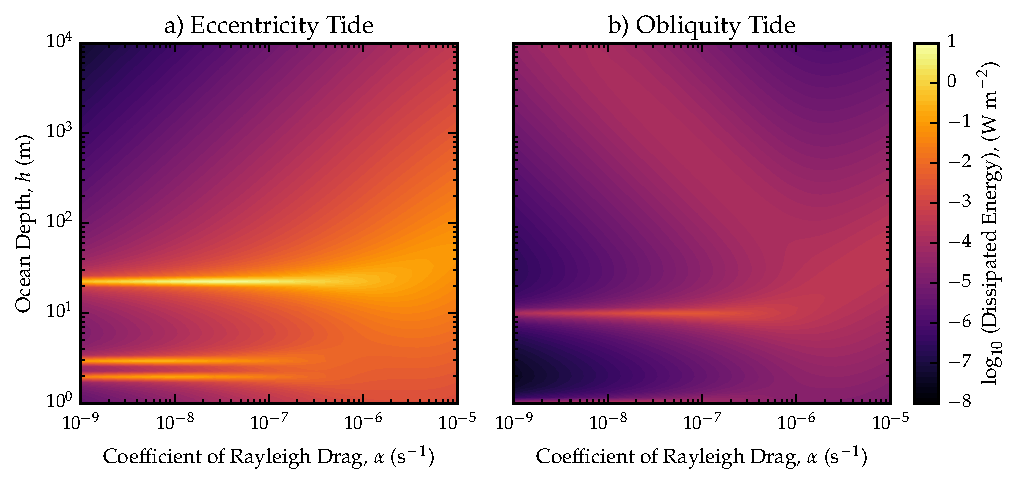
\includegraphics[width=\linewidth]{Figures/titan_linear}
        \phantomcaption
        \label{fig:lincEccTitan}
    \end{subfigure}
    \begin{subfigure}[t]{0\linewidth} % the hidden unwanted image
         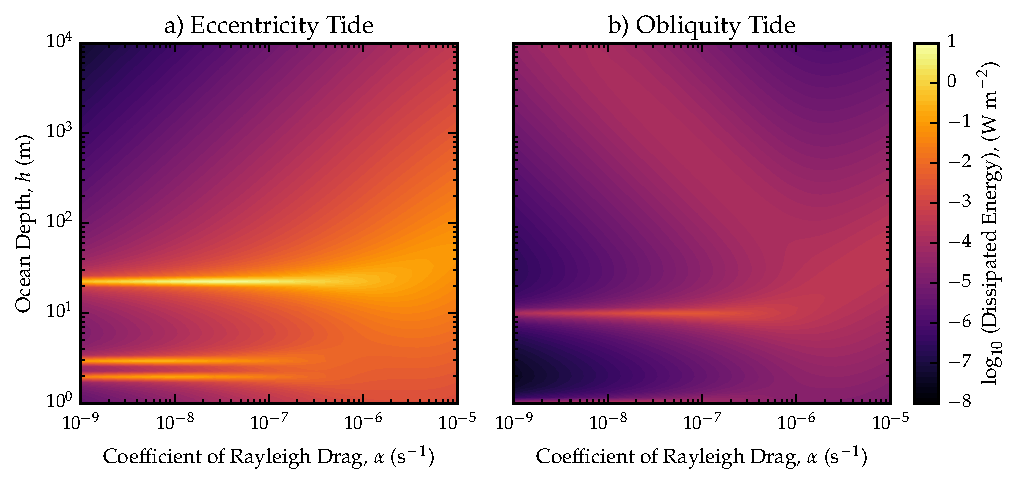
\includegraphics[width=\linewidth]{Figures/titan_linear}
         \phantomcaption
         \label{fig:linObliqTitan}   
    \end{subfigure}
    \vspace{-0.5cm}
\caption{Global ocean surface dissipation solution for Titan under the eccentricity (left) and obliquity (right) tides. The logarithm of dissipated energy is shown as a function of ocean depth, $h$, and Rayleigh drag coefficient, $\alpha$. All simulations were performed with \SIrange{2}{3}{\degree} resolution.}
\label{fig:linTitan}
\end{figure*}

\section{Ocean Dissipation in Titan \label{sec:results_Titan}}

The following results are split into three main sections. Firstly, we compare dissipation between Rayleigh (section \ref{sec:ray_titan}) and bottom (section \ref{subsec:botTitan}) drag for Titan. Section \ref{subsec:scalTitan} then compares the bottom drag results to scaling laws from \citet{chen2013tidal}. We repeat these results for Enceladus in section \ref{sec:results_Enceladus}.

\subsection{Rayleigh Drag}\label{sec:ray_titan}

Dissipated surface heat flux averaged over the tidal period was calculated for over 3000 simulations over $h$ and $\alpha$ space for each main tidal component, as shown in Figure \ref{fig:linTitan}. The eccentricity tide (Figure \ref{fig:lincEccTitan}) shows three resonant ocean thicknesses, $h \sim$ \SIlist{2;3;22}{\metre}. These horizontal resonances are the result of excited gravity waves, with the deepest of these having a maximum dissipated surface heat flux of $\sim 10\, \si{\watt\per\square\metre}$ which occurs between $\alpha =$ \SIrange{e-8}{e-7}{\per\second}. Notably, the maximum dissipated energy does not occur for the most drag dominated oceans where $\alpha \sim \num{e-5} \, \si{\per\second}$. 

\begin{figure*}[!t]
    \centering
    \begin{subfigure}[t]{0.85\linewidth} % contains the two plots in a single figure
        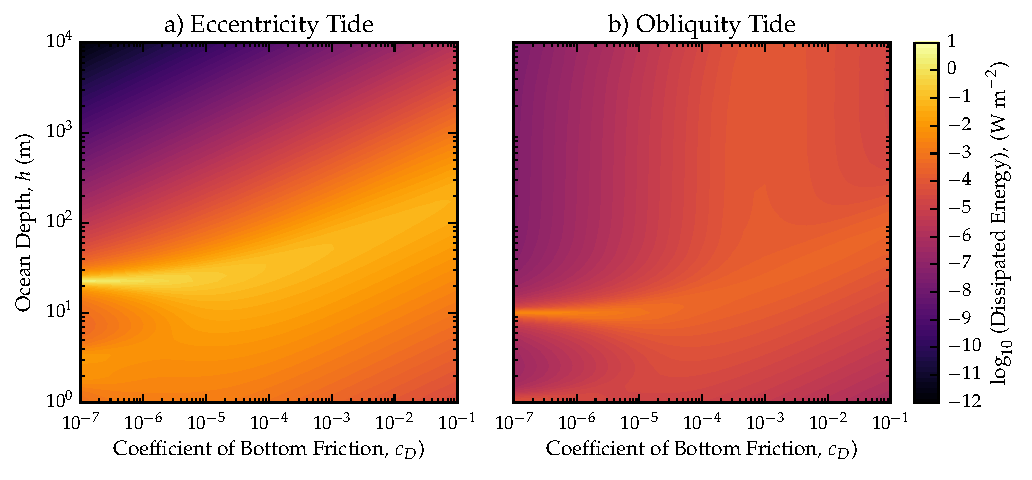
\includegraphics[width=\linewidth]{Figures/titan_bottom}
        \phantomcaption
        \label{fig:botEccTitan}
    \end{subfigure}
    \begin{subfigure}[t]{0\linewidth} % the hidden unwanted image
         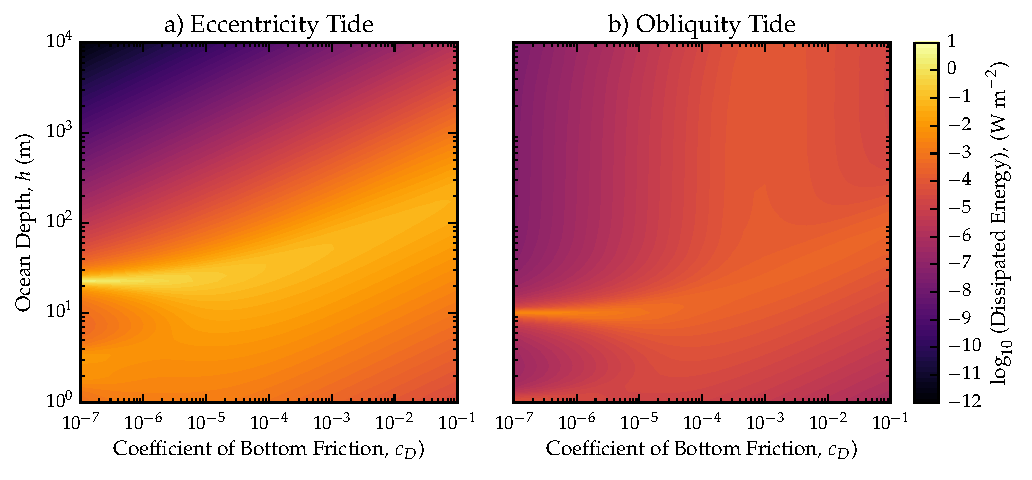
\includegraphics[width=\linewidth]{Figures/titan_bottom}
         \phantomcaption
         \label{fig:botObliqTitan}   
    \end{subfigure}
    \vspace{-0.5cm}
\caption{Global ocean surface dissipation solution for Titan under the eccentricity (left) and obliquity (right) tides. The logarithm of dissipated energy is shown as function of ocean depth, $h$, and coefficient of bottom drag, $c_D$. All simulations were performed with \SIrange{1}{3}{\degree} resolution. \label{fig:botTitan}}
\end{figure*}


Figure \ref{fig:linObliqTitan} illustrates the dissipated surface heat flux for the obliquity tide on Titan. Two resonant ocean thicknesses are found for this tidal component, $h \sim$ \SIlist{1;10}{\metre}. The latter resonance is the most dissipative with an average surface heat flux of $\sim \num{4e-3}\, \si{\watt\per\square\metre}$. There is also an excited Rossby wave resonance orientated diagonally across $h \sim$ \SIrange{10}{e4}{\metre} and \hbox{$\alpha \sim$ \SIrange{e-6}{e-9}{\per\second}}. The average surface heat flux occurring along the length of this resonance is $\sim \SI{e-4}{\watt\per\square\metre}$. 

Numerical error was also computed using the semi-analytical solutions from \citep{matsuyama2014tidal}. The eccentricity tide is accurate to within 1\% over much of the parameter space, with resonances being the least accurate (in terms of absolute value). The deepest resonance differs from the analytical solution by \SIrange{1}{20}{\percent}. We ignore discrepancies in shallow oceans ($h_0 \leq 10 \, \si{\metre}$) as bathymetry of the ocean floor for any icy satellite will likely be comparable to or exceed the depth of such a thin the ocean, directly violating the assumptions made in the LTEs. It should also be noted that resonances found below $h_0 = 10 \, \si{\metre}$ typical have displacements greater than the depth of the ocean itself, another violation of the LTEs assumptions. As such, we deem this part of the parameter space unphysical.

\subsection{Bottom Drag \label{subsec:botTitan}}

Dissipation across $h$ and $c_D$ space (bottom drag) is shown in Figure \ref{fig:botTitan}. Tidal dissipation due to the eccentricity tide is shown in the left hand figure. Comparing this to Rayleigh dissipation in Figure \ref{fig:lincEccTitan} highlights some of the major differences and similarities between the two drag regimes. The resonant peaks at \SIlist{2;3;22}{\metre} from the Rayleigh drag case are all present, although they have smaller magnitudes. The resonance broadens towards larger $c_D$, and remains very diffuse over much of the parameter space. This differs from the Rayleigh drag case where the resonances are very narrow and pronounced over most of $\alpha$ space (Figure \ref{fig:lincEccTitan}). Additionally, away from the resonances and in the deepest oceans, dissipated energy drops by \numrange{10}{12} orders of magnitude when applying bottom drag, which is far smaller than the lowest dissipation found in the Rayleigh drag case.  

Ocean dissipation under the obliquity tide using bottom drag also has several important differences and similarities to the Rayleigh case. Comparing figures \ref{fig:botObliqTitan} and \ref{fig:linObliqTitan}, it is again evident that the horizontal gravity wave resonances at \SIlist{1;10}{\metre} are present in both solutions. Perhaps the most significant difference between each case is the orientation of the broad resonance that extends to the deepest oceans. In the Rayleigh case, this resonance moves diagonally across a large region of the parameter space, whereas it is vertically oriented and limited to a small range of $c_D$ for the bottom drag case, such that the resonance becomes independent of ocean depth. The resonance also happens to occur across the empirically derived Earth value for $c_D = 0.002$ \citep[e.g.,][]{sohl1995tidal,egbert2001estimates}. %Unlike in the Rayleigh case, these resonances rapidly broaden towards higher $c_D$, when bottom drag becomes more dominant

\subsection{Comparison with Scaling Laws \label{subsec:scalTitan}}

\begin{figure*}[!t]
\centering
\begin{subfigure}{0.5\linewidth}
\centering
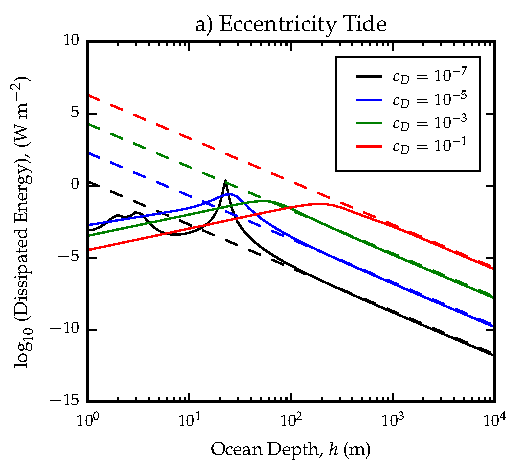
\includegraphics[width=0.85\linewidth]{Figures/Eccentricity_scaling}
\subcaption{\label{fig:scalEccTitan}}
\end{subfigure}%
\begin{subfigure}{0.5\linewidth}
\centering
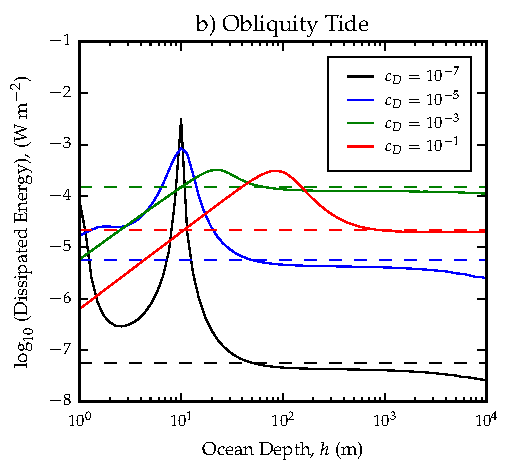
\includegraphics[width=0.85\linewidth]{Figures/Obliquity_scaling}
\subcaption{\label{fig:scalObliqTitan}}
\end{subfigure}
\vspace*{-0.8cm}
\caption{Comparison of the ODIS numerical results (solid lines) and those calculated using the scaling laws (dashed lines) derived in \citet{chen2013tidal}, for Titan under the eccentricity (left) and obliquity (right) tides. The colours represent different values of bottom drag coefficient.\label{fig:scalTitan}}
\end{figure*}

While there are no fully analytical solutions to the LTEs when including bottom drag, there are a set of scaling laws for estimating dissipation that neglect gravity wave resonant features, developed by \citet{chen2013tidal}. We compare cross sections from the results in Figure \ref{fig:botTitan} with these scaling laws, shown in Figure \ref{fig:scalTitan}.

Away from resonances and in deep oceans, there is excellent agreement between the numerical results and the scaling laws. This is particularly true of the eccentricity tide. Larger discrepancies are found for the obliquity tide (Figure \ref{fig:scalObliqTitan}) for deep oceans, but this is a result of discretisation error. The vertically orientated resonant feature in Figure \ref{fig:botObliqTitan} is also produced from the scaling laws, as shown in Figure \ref{fig:scalObliqTitan}. None of the gravity wave resonances are captured by the scaling laws. 

\subsection{Implications for Titan}

Titan likely has an ocean that is on the order of \SI{100}{\kilo\metre} thick \citep{sohl2014structural,baland2014titan}. All of the eccentricity tide resonances occur at ocean depths much shallower than this, suggesting that - despite the substantial free eccentricity - there is little dissipation from this tidal component in heating Titan's ocean.

Rossby wave resonances from the obliquity tide appear as the diagonal and vertical features in figures \ref{fig:linObliqTitan} and \ref{fig:botObliqTitan}, respectively. The linear drag resonance moves into unrealistically low Rayleigh drag coefficients ($\alpha \lesssim$ \SI{e-9}{\per\second}) for oceans deeper than about \SI{10}{\kilo\metre}. However, for bottom drag, the Rossby wave resonance is mainly independent of ocean depth above $h \gtrsim$ \SI{1}{\kilo\metre}. If Titan's ocean fell within the $c_D =$ \SIrange{e-2}{e-4} range then this Rossby wave resonance could provide a non-neglible thermal energy component to Titan's interior, regardless of the ocean depth. To gain some insight into how significant this dissipation can be, we consider some upper limits of Titan's semimajor axis evolution.

Hyperion is the next furthest satellite from Saturn after Titan, with a semimajor axis  \num{1.23} times that of Titan's (taken from the JPL satellite ephemerides: \url{http://ssd.jpl.nasa.gov/?sat_elem}). Titan would had to have originated at some semimajor axis less than Hyperion's, otherwise Hyperion would have been disturbed or ejected from the system, assuming Hyperion and Titan have similar ages. This provides us with a useful upper bound on Titan's  initial semimajor axis. Using the dissipated energy results for the obliquity tide under bottom drag we can examine how rapidly Titan's semimajor axis shrinks to its present day value.

For a bound orbit the total energy is given as $-GMm/2a$ \citep{murray1999solar}. Differentiating this expression with respect to time gives a relationship between the dissipated energy and changing semimajor axis,
\begin{equation}
\dot{a} = \dfrac{2a^2 \dot{E}}{GM m}.
\label{eq:adot}
\end{equation}

where $M$ and $m$ represent the mass of Saturn and Titan, respectively. The universal gravitational constant is $G$, and dissipated energy is $\dot{E}$. Note that as $\dot{E} < 0$, the semimajor axis decays with time. To first order, we find that $\dot{E}$ remains nearly constant over the range $1.21 a$ to $a$ for a deep ocean on Titan experiencing bottom drag for the obliquity tide. This is because the position of the vertical Rossby wave resonance (Figure \ref{fig:botObliqTitan}) is sensitive to the rotation rate of Titan, which hardly varies from $\Omega =$ \SIrange{4.56e-6}{3.42e-6}{\per\second} over the range of semimajor axes that we consider, assuming synchronous rotation. We are thus able to set $\dot{E}$ to constant in the following calculations. Additionally, it should be noted that while $\dot{E}$ is rather sensitive to the actual obliquity, $\theta_0$, we set the obliquity to constant over time for simplicity. A more rigorous (and future) approach would include the coupling between energy and obliquity.

\begin{figure}[!b]
\centering
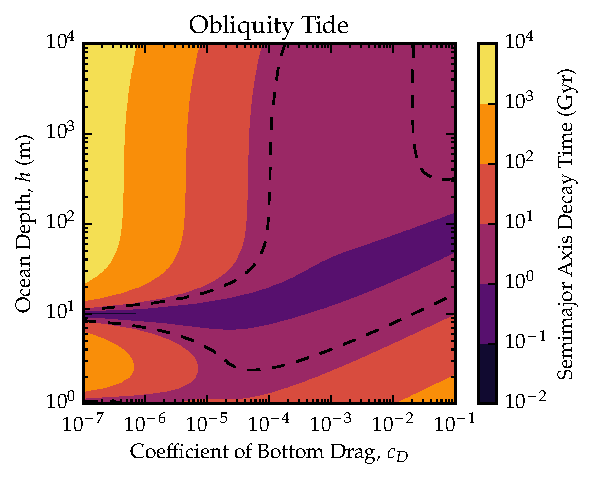
\includegraphics[width=\linewidth]{Figures/titan_timescale}
\caption{Semimajor axis decay timescale, $\tau_a$, as a function of ocean depth and bottom drag coefficient for the obliquity tide on Titan. This timescale represents the time taken for the semimajor axis of Titan to shrink from that of Hyperion's to the present day value. The dashed contour represents the age of the Solar System, $\sim \SI{4.5}{\giga\year}$. \label{fig:a_evo}}
\end{figure}

\begin{figure*}[!t]
    \centering
    \begin{subfigure}[t]{0.85\linewidth} % contains the two plots in a single figure
        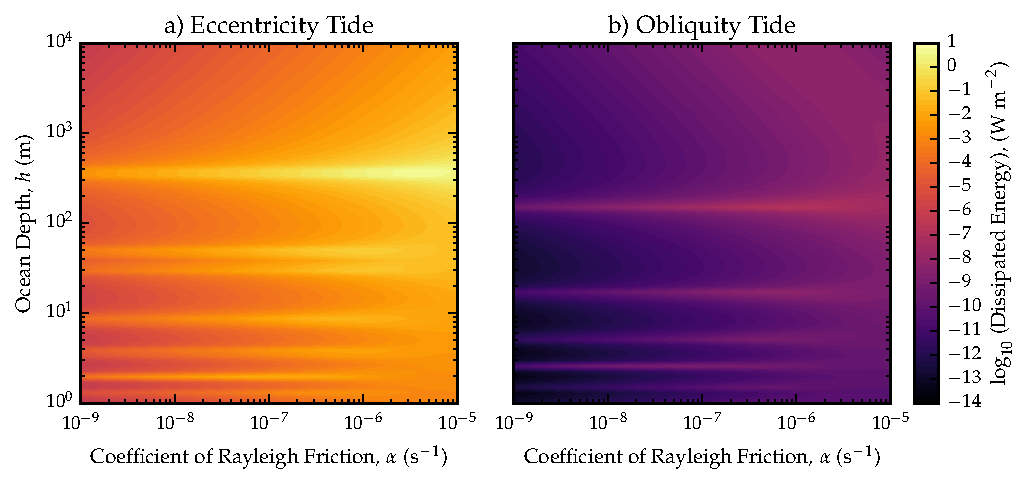
\includegraphics[width=\linewidth]{Figures/enceladus_linear}
        \phantomcaption
        \label{fig:lincEccEncel}
    \end{subfigure}
    \begin{subfigure}[t]{0\linewidth} % the hidden unwanted image
         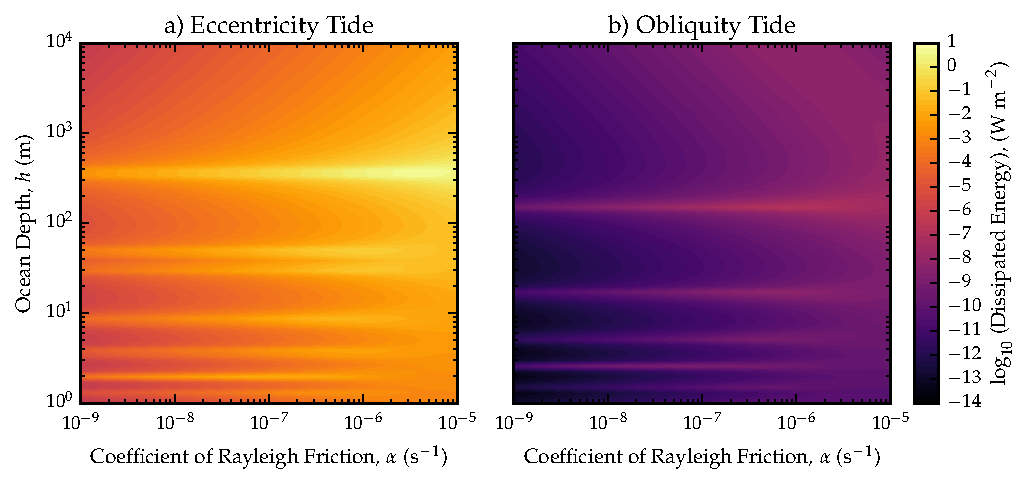
\includegraphics[width=\linewidth]{Figures/enceladus_linear}
         \phantomcaption
         \label{fig:linObliqEncel} 
    \end{subfigure}
    \vspace{-0.5cm}
\caption{Time and surface averaged ocean dissipation for Enceladus under the eccentricity (left) and obliquity (right) tides when applying Rayleigh drag. The logarithm of dissipated energy is shown as function of ocean depth, $h$, and bottom drag coefficient, $c_D$. All simulations were performed with \SIrange{1}{3}{\degree} grid resolution. \label{fig:linEncel}}
\end{figure*}

We integrate Equation \ref{eq:adot} to estimate the evolution of Titan's semimajor axis as a function of time and dissipated energy, defining a characteristic semimajor axis decay time, $\tau_{a}$, as the time taken for the semimajor axis to reach its present day value from Hyperion's. The decay time as a function of ocean depth and bottom drag coefficient is shown in Figure \ref{fig:a_evo}.
  
As expected, the smallest $\tau_a$ occurs for the largest dissipation, namely the gravity wave resonance at \SI{10}{\metre}, with decay times on the order of \SIrange{10}{100}{\mega\year}. However, as previously mentioned, Titan's ocean is likely in excess of \SI{100}{\kilo\metre} thick, and is thus far from this resonance. Figure \ref{fig:a_evo} shows that for ocean depths $h_0 >$ \SI{1}{\kilo\metre} the decay time-scale (and dissipation) is effectively independent of ocean depth. Although not shown, this behaviour continues right up to the shallow water limit ($h_0 \lesssim 0.1r$) as predicted by the \citet{chen2013tidal} scaling laws. Thus, for $c_D =$ \SIrange{e-4}{2e-2}, Titan's semimajor axis would shrink to its present day value in less than the age of the Solar System ($\sim$\SI{4.5}{\giga\year}, denoted by the dashed contour in Figure \ref{fig:a_evo}). If Titan's orbit originated with a semimajor axis between its current value and less than Hyperion's value, then we would expect Titan to have a smaller semimajor axis than that observed today.

Although the initial value of $a$ is not known, the scenario described above is not consistent with the deep ocean estimates of \citet{sohl2014structural, baland2014titan} if we assume a bottom drag coefficient within an order of magnitude of the canonical Earth value ($c_D =$ \num{0.002}). Instead, our estimates of the decay time-scale suggest that Titan's ocean has a bottom drag coefficient of \hbox{$ \num{e-4} \gtrsim c_D \gtrsim \num{2e-2} $}. These constraints indicate that Titan's ocean experiences anomalously low or high drag (not dissipation) than compared to the Earth's ocean.

Titan is a very slow rotator, resulting in limited ocean flow. This factor reduces the amount of turbulent bottom flow experienced in the ocean, consequently lowering the bottom drag coefficient. This is consistent with the low drag limit. However, one could additionally argue that the presence of a solid lid, although neglected here, would result in an extremely turbulent ``top'' drag environment, consistent with the high drag limit. At present there is not sufficient evidence to favour one of these limits over the other and should be a focus of future work.  

Although we do not attempt to compute the eccentricity evolution (which is far more challenging with non-radial tidal components), the almost negligible amount of dissipated energy for $h_0 >$ \SI{1}{\kilo\metre} shown in Figure \ref{fig:botObliqTitan} should allow Titan to maintain its relatively high free eccentricity of 0.0288. Here we of course neglect dissipation in Titan's solid interior.
\section{Ocean Dissipation in Enceladus \label{sec:results_Enceladus}}

\subsection{Rayleigh Friction} \label{sec:ray_enc}

As with our Titan results, we calculated globally averaged surface heat flux for over 3000 simulations in the $h$-$\alpha$ parameter space. These results are shown for the eccentricity and obliquity tides in Figure \ref{fig:linEncel}.

There are several more gravity wave resonances found for Enceladus than Titan in both tidal components, as shown in Figure \ref{fig:lincEccEncel}. The eccentricity tide excites resonances at \SIlist{1.3;1.9;3.8;8.7;29;50;360}{m}; a total of 7 resonances, whereas Titan only has 3 (Figure \ref{fig:lincEccTitan}). By solving the LTEs using both the eccentricity-radial and libration tides simultaneously, we capture any coupling these two tidal components may initiate in the ocean flow and find no new resonances. Increasing the resolution of the parameter space would almost certainly reveal more resonances, but this is only likely for oceans with $h_0 <$ \SI{10}{\metre}. 

The most dissipative eccentricity tide resonance is also the deepest, with an average surface heat flux of \SI{4.6}{\watt\per\square\metre} at $\alpha\sim$ \SI{2e-6}{\per\second}, three orders of magnitude greater than Titan's largest resonance. This is equivalent to a total power output of $\sim$ \SI{3610}{\giga\watt}, well in excess of the observed value of (at least) \SI{5}{\giga\watt} by two to three orders of magnitude \citep{spencer2006cassini,howett2011high, spencer2013new}.  

\begin{figure}[!t]
    \centering
    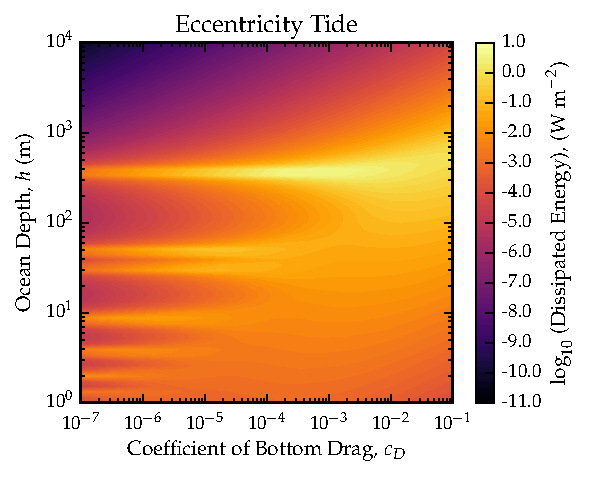
\includegraphics[width=\linewidth]{Figures/enceladus_bottom}
\caption{As for Figure \ref{fig:linEncel}, but for the bottom drag regime. The obliquity tide is also ignored. \label{fig:botEncel}}
\end{figure}

The stark colour difference between the eccentricity and obliquity tide plots in Figure \ref{fig:linEncel} is a result of Enceladus' negligible obliquity ($\theta_0 \sim$ \num{e-4} degrees \citep{chen2013tidal, baland2016obliquity}). This causes average surface dissipation to range from \SIrange{e-7}{e-14}{\watt\per\square\metre} over our explored parameter space, which has an almost negligible effect on the thermal and orbital evolution of the satellite. Gravity wave resonances are found at \SIlist{1.6;2.7;5.5;18;160}{\metre}, with the characteristic Rossby wave resonance extending diagonally across the parameter space from around $h=$ \SI{500}{\metre}.

Away from shallow oceans, we once again find excellent agreement between the numerical and semi-analytical solutions from \citet{matsuyama2014tidal} in terms of both the resonant ocean thicknesses and magnitude of the dissipation. Much of the parameter space has a discrepancy of $<$ \SIrange{1}{5}{\percent}, with this increasing to $\sim$ \SI{10}{\percent} for resonances. As demonstrated in Figure \ref{fig:conv}, this can easily be decreased with higher resolution simulations, at the expense of computational run time.


\subsection{Bottom Friction}

We neglect running the obliquity tide bottom drag case for Enceladus. As mentioned in the previous section, the obliquity of Enceladus is close to Cassini State \citep{chen2011obliquity,chen2013tidal}, making tidal flow and dissipation from obliquity negligible. Additionally, the low drag experienced due to weak obliquity tide flow leads to long simulation run times in order to achieve equilibrium, which is a severe challenge numerically.

Bottom drag results for the eccentricity tide on Enceladus are shown in Figure \ref{fig:botEncel}. The gravity wave resonances are found at identical ocean thicknesses to the Rayleigh drag results in Figure \ref{fig:lincEccEncel}. There is, however, a much greater contrast in dissipation magnitude in this parameter space when compared to the Rayleigh drag results. Dissipation drops off rapidly by many orders of magnitude with increasing ocean depth away from the \SI{360}{\metre} resonance. This is expected given the velocity squared dependence in the bottom drag term in Equation \ref{eq:mom}. 

\subsection{Comparison with Scaling Laws}

\begin{figure}[!b]
\centering
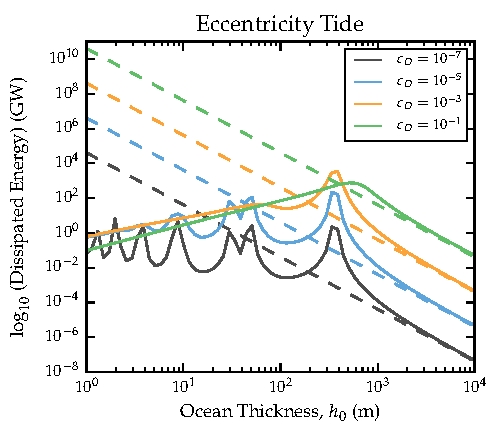
\includegraphics[width=0.85\linewidth]{Figures/enceladus_scaling}
\caption{Comparison of the ODIS numerical results (solid lines) and those calculated using the scaling laws (dashed lines) derived in \citet{chen2013tidal}, for Enceladus under the eccentricity tide. The colours represent different values of bottom drag coefficient. \label{fig:scalEncel}}
\end{figure}

The bottom drag eccentricity tide results for Enceladus are compared to \citet{chen2013tidal} scaling laws in Figure \ref{fig:scalEncel}. As was the case with Titan, we find poor agreement for resonant ocean configurations, with increasingly good agreement away from resonances. The scaling laws cannot take into account the resonant ocean configurations due to the non-linearity of these features. However, the general trend of decreasing dissipation with increasing ocean depth is captured by the scaling laws and agrees well with our numerical results. This agreement provides further validation to the numerical model and techniques employed in this work.

\subsection{Implications for Enceladus}

Eccentricity is the only significant contributor to ocean dissipation in Enceladus. Under both Rayleigh and bottom drag, the deepest occurring gravity wave resonance can easily account for the observed SPT power output \citep{spencer2006cassini,howett2011high,spencer2013new}. However, this resonance is relatively shallow. Of course, Enceladus' ocean depth is unconstrained, although non-unique gravity modelling is consistent with an ocean on the order of \SI{10}{\kilo\metre} thick, at least under the SPT \citep{iess2014gravity}. Thus, based on our results, we expect that ocean dissipation is insignificant over long time scales for Enceladus. 
%Resonant ocean configurations occur only for shallow oceans under the eccentricity tide and obliquity tide flow is negligible, meaning dissipation is minimal over the vast majority of the likely parameter space.

The numerical model has also revealed no new resonances in either Rayleigh or bottom drag by applying both the eccentricity-radial and eccentricity-libration tide simultaneously, a technique that is not possible analytically.

The amplitude of forced libration on Enceladus \citep{thomas2015enceladus}, as well as the negative mass anomaly observed at the SPT \citep{iess2014gravity, mckinnon2015effect} indicate that its subsurface ocean is global in extent and deeper beneath the SPT. This variable ocean thickness is neglected in our model, and may lead to localised heating at the boundary between shallow and deep oceans. The effect on resonance ocean configurations is unknown. Incorporating a variable ocean thickness into the LTEs is only possible numerically, and will be one focus of future work.




%\section{Discussion \label{sec:discussion}}



\section{Conclusions}

We have designed and implemented a numerical model based on \citet{sears1995tidal} to solve the dissipative Laplace Tidal Equations on a sphere. This model, valid only in the shallow water limit and assuming a global surface ocean, has been used to model ocean flow and its associated tidal dissipation over a range of ocean thicknesses and drag coefficients for both Titan and Enceladus. We neglect the effects of ocean loading and self-attraction.

Modelling is performed with both Rayleigh (linear) and bottom (quadratic) drag models. The former represents internal drag between two adjacent fluid parcels \citep{neumann1968ocean}, while the latter is a global scale approach to incorporating the effects of a macro-scale turbulent boundary layer at some solid-fluid interface \citep{gill1982atmosphere}.

Rayleigh drag results were compared to that of \citet{matsuyama2014tidal} yielding mostly excellent agreement over much of the explored parameter space, providing important validation to our numerical model. Ocean dissipative resonances were replicated well in both Rayleigh and bottom drag simulations. Importantly, we have also demonstrated good agreement between our bottom drag numerical results and the scaling laws of \citet{chen2013tidal} away from gravity-wave resonances, providing further validation of the bottom drag implementation in our model.

For Titan, all gravity-wave resonances occur in very thin oceans and as such  are unlikely to exist. The exception is the Rossby-wave resonance associated with the obliquity tide, which becomes independent of ocean thickness away from thin oceans ($h_0 \leqslant\SI{1}{\kilo\metre}$) in the bottom drag regime. This is also shown in the \citet{chen2013tidal} obliquity tide scaling law. Such a feature means that for a thick ocean on Titan, which is thought to be the case \citep{sohl2014structural}, ocean dissipation becomes dependent on only bottom drag coefficient. For an Earth like bottom drag coefficient we find that ocean dissipation induced by Titan's obliquity tide can reduce its rate of outward orbital migration by  $\sim\SI{40}{\percent}$. Additionally, measurement of $da/dt$ could place constraints on the bottom drag coefficient of Titan's ocean because this resonance becomes independent of ocean thickness. 

Characteristic eccentricity decay times scales for a thick ocean on Titan are found to be well in excess of the age of the Solar System. This is consistent with the relatively high eccentricity observed for Titan at the present day. Any eccentricity damping must therefore come from alternate sources, such as dissipation in the solid regions of the satellite.

Enceladus' eccentricity tide ocean resonances are found to be extremely dissipative, as in \citet{tyler2011tidal, matsuyama2014tidal}. However, the ocean thicknesses where these resonances form are almost certainly too small to be present on Enceladus. We hope to model tidal flow for a spatially varying ocean thickness on Enceladus in the future, as this will likely effect resonant thicknesses and may lead to more localised heating at the SPT. Additionally, it is important to incorporate a solid icy lid into our model to understand how this affects ocean dynamics and dissipation, which will be explored in future work. 

\section*{References}
\bibliography{mybibfile}

%\appendix

\section{Laplace Tidal Equations in Spherical Coordinates \label{app:coords}}

To convert the Laplace Tidal Equations to a spherical coordinate system we must make use of the following well-known identities for the gradient and divergence operators,
\begin{equation}
\nabla f = \frac{1}{R} \partial_{\lambda} f \bm{\hat{\lambda}}  
+ \frac{1}{R \cos{\lambda}} \partial_{\lambda} f \bm{\hat{\phi}}
\end{equation}
\begin{equation}
\nabla \cdot \bm{A} = -\frac{1}{R \cos{\lambda}} \partial_{\lambda} \left( \cos{\lambda}\, A_{\lambda} \right) + \frac{1}{R \cos{\lambda}} \partial_{\phi} A_{\phi}
\end{equation}

where $\bm{A}$ is some vector quantity tangent to the spherical surface, $f$ is a scalar quantity, and $\bm{\hat{\lambda}}$ and $\bm{\hat{\phi}}$ are the latitude and longitude unit vectors, also tangent to the surface.
Defining $\bm{u} = \left(u, v \right) = (u_{\phi}, -u_{\lambda} ) $ and using the fact that $\bm{\Omega} = \Omega \bm{\hat{k}}$, where $\bm{\hat{k}}$ is the cartesian unit vector aligned with the rotation axis, then the continuity equation can be rewritten as,
\begin{equation}
\partial_t \eta + \frac{h_0}{R \cos{\lambda}} \left( \partial_{\lambda}
\left(v \cos{\lambda} \right) +  \partial_{\phi} u \right) = 0 \, .
\end{equation}

\noindent Similarly, the momentum equation becomes, 
\begin{equation}
\partial_t u - 2 \Omega v \sin{\lambda}
+ \alpha u
+\frac{c_D}{h_0} \left(u^2 + v^2 \right)^{\nicefrac{1}{2}} u
+ \frac{g}{R \cos{\lambda}} \partial_{\phi} \eta
= 
(1 + k_2 - h_2) \frac{1}{R \cos{\lambda}} \partial_{\phi} U_2
\end{equation}
\begin{equation}
\partial_t v + 2 \Omega u \sin{\lambda}
+ \alpha v
+\frac{c_D}{h_0} \left(u^2 + v^2 \right)^{\nicefrac{1}{2}} v
+ \frac{g}{R} \partial_{\lambda} \eta
= 
(1 + k_2 - h_2) \frac{1}{R} \partial_{\lambda} U_2
\end{equation}

%
%\section{Finite Difference Energy Expressions \}
%
%For a system experiencing both Rayleigh and bottom friction, the full dissipated energy over an orbit is given by,
%\begin{equation}
%F = \frac{\rho}{4 \pi T} \iint \left[h \alpha \left(u^2 + v^2 \right) + c_D \left(u^2 + v^2 \right)^\nicefrac{3}{2} \right}d\Omega dt,
%\end{equation}
%
%\noindent where $\Omega$ is the solid angle and we assume that $h \ll R$.


\end{document}
